\documentclass[12pt]{article}

\usepackage{amsmath, mathtools}
\usepackage{amsfonts}
\usepackage{amssymb}
\usepackage{graphicx}
\usepackage{colortbl}
\usepackage{xr}
\usepackage{hyperref}
\usepackage{longtable}
\usepackage{xfrac}
\usepackage{tabularx}
\usepackage{float}
\usepackage{siunitx}
\usepackage{booktabs}
\usepackage{caption}
\usepackage{pdflscape}
\usepackage{afterpage}
\usepackage{subfig}

\usepackage[round]{natbib}

%\usepackage{refcheck}

\hypersetup{
    bookmarks=true,         % show bookmarks bar?
      colorlinks=true,       % false: boxed links; true: colored links
    linkcolor=red,          % color of internal links (change box color with linkbordercolor)
    citecolor=green,        % color of links to bibliography
    filecolor=magenta,      % color of file links
    urlcolor=cyan           % color of external links
}

%% Comments

\usepackage{color}

\newif\ifcomments\commentstrue %displays comments
%\newif\ifcomments\commentsfalse %so that comments do not display

\ifcomments
\newcommand{\authornote}[3]{\textcolor{#1}{[#3 ---#2]}}
\newcommand{\todo}[1]{\textcolor{red}{[TODO: #1]}}
\else
\newcommand{\authornote}[3]{}
\newcommand{\todo}[1]{}
\fi

\newcommand{\wss}[1]{\authornote{blue}{SS}{#1}} 
\newcommand{\plt}[1]{\authornote{magenta}{TPLT}{#1}} %For explanation of the template
\newcommand{\an}[1]{\authornote{cyan}{Author}{#1}}

%% Common Parts

\newcommand{\progname}{AortaGeomRecon} % PUT YOUR PROGRAM NAME HERE
\newcommand{\authname}{Jingyi Lin} % AUTHOR NAMES                  

\usepackage{hyperref}
    \hypersetup{colorlinks=true, linkcolor=blue, citecolor=blue, filecolor=blue,
                urlcolor=blue, unicode=false}
    \urlstyle{same}
                                


% For easy change of table widths
\newcommand{\colZwidth}{1.0\textwidth}
\newcommand{\colAwidth}{0.13\textwidth}
\newcommand{\colBwidth}{0.82\textwidth}
\newcommand{\colCwidth}{0.1\textwidth}
\newcommand{\colDwidth}{0.05\textwidth}
\newcommand{\colEwidth}{0.8\textwidth}
\newcommand{\colFwidth}{0.17\textwidth}
\newcommand{\colGwidth}{0.5\textwidth}
\newcommand{\colHwidth}{0.28\textwidth}

% Used so that cross-references have a meaningful prefix
\newcounter{defnum} %Definition Number
\newcommand{\dthedefnum}{GD\thedefnum}
\newcommand{\dref}[1]{GD\ref{#1}}
\newcounter{datadefnum} %Datadefinition Number
\newcommand{\ddthedatadefnum}{DD\thedatadefnum}
\newcommand{\ddref}[1]{DD\ref{#1}}
\newcounter{theorynum} %Theory Number
\newcommand{\tthetheorynum}{T\thetheorynum}
\newcommand{\tref}[1]{T\ref{#1}}
\newcounter{tablenum} %Table Number
\newcommand{\tbthetablenum}{T\thetablenum}
\newcommand{\tbref}[1]{TB\ref{#1}}
\newcounter{assumpnum} %Assumption Number
\newcommand{\atheassumpnum}{P\theassumpnum}
\newcommand{\aref}[1]{A\ref{#1}}
\newcounter{goalnum} %Goal Number
\newcommand{\gthegoalnum}{P\thegoalnum}
\newcommand{\gsref}[1]{GS\ref{#1}}
\newcounter{instnum} %Instance Number
\newcommand{\itheinstnum}{IM\theinstnum}
\newcommand{\iref}[1]{IM\ref{#1}}
\newcounter{reqnum} %Requirement Number
\newcommand{\rthereqnum}{P\thereqnum}
\newcommand{\rref}[1]{R\ref{#1}}
\newcounter{nfrnum} %NFR Number
\newcommand{\rthenfrnum}{NFR\thenfrnum}
\newcommand{\nfrref}[1]{NFR\ref{#1}}
\newcounter{lcnum} %Likely change number
\newcommand{\lthelcnum}{LC\thelcnum}
\newcommand{\lcref}[1]{LC\ref{#1}}
\newcounter{ucnum} %Unlikely change number
\newcommand{\ltheucnum}{UC\theucnum}
\newcommand{\ucref}[1]{UC\ref{#1}}

\usepackage{fullpage}

\newcommand{\deftheory}[9][Not Applicable]
{
\newpage
\noindent \rule{\textwidth}{0.5mm}

\paragraph{RefName: } \textbf{#2} \phantomsection 
\label{#2}

\paragraph{Label:} #3

\noindent \rule{\textwidth}{0.5mm}

\paragraph{Equation:}

#4

\paragraph{Description:}

#5

\paragraph{Notes:}

#6

\paragraph{Source:}

#7

\paragraph{Ref.\ By:}

#8

\paragraph{Preconditions for \hyperref[#2]{#2}:}
\label{#2_precond}

#9

\paragraph{Derivation for \hyperref[#2]{#2}:}
\label{#2_deriv}

#1

\noindent \rule{\textwidth}{0.5mm}

}

\begin{document}

\title{Software Requirements Specification for \progname{}} 
\author{\authname}
\date{\today}
	
\maketitle

~\newpage

\pagenumbering{roman}

\tableofcontents

~\newpage

\section*{Revision History}

\begin{tabularx}{\textwidth}{p{3cm}p{2cm}X}
\toprule {\bf Date} & {\bf Version} & {\bf Notes}\\
\midrule
2023-02-12 & 1.0 & Notes\\
\midrule
2023-03-01 & 1.01 & Modified system context image, coordinate systems, and goal statements.\\
\midrule
2023-04-29 & 1.02 & Added requirements, instance models, data definitions\\
\midrule
2023-06-05 & 1.03 & Added Traceability Matrices \\
\midrule
2023-06-18 & 1.04 & Include the missing sections, modified the equations of DD, and IM. Added 4 new NFRs.\\
\bottomrule
\end{tabularx}

~\newpage

\section{Reference Material}

This section records information for easy reference.

\subsection{Table of Units}

Throughout this document SI (Syst\`{e}me International d'Unit\'{e}s) is employed
as the unit system.  In addition to the basic units, several derived units are
used as described below.  For each unit, the symbol is given followed by a
description of the unit and the SI name.

\subsection{Table of Symbols}

The table that follows summarizes the symbols used in this document along with
their units.  The choice of symbols was made to be consistent with existing documentation for 3D Slicer program. 
The symbols are listed in alphabetical order.

\renewcommand{\arraystretch}{1.2}
\noindent \begin{longtable}{l p{2cm} p{12cm}} \toprule
  \textbf{symbol} & \textbf{type} & \textbf{description}\\
  \midrule
\textit{m} & $\mathbb{N}$ &  The first dimension of the segmentation volume.
\\
\textit{m}$_{i}$ & $\mathbb{N}$ &  The first dimension of \textit{V}$_\text{in}$.
\\
\textit{m}$_{o}$ & $\mathbb{N}$ &  The first dimension of \textit{V}$_\text{out}$.
\\
\textit{n} & $\mathbb{N}$ &  The second dimension of the segmentation volume.
\\
\textit{n}$_{i}$& $\mathbb{N}$ &  The second dimension of \textit{V}$_\text{in}$.
\\
\textit{n}$_{o}$ & $\mathbb{N}$ &  The second dimension of \textit{V}$_\text{out}$.
\\
\textit{p} & $\mathbb{N}$ &  The third dimension of the segmentation volume.
\\
\textit{p}$_{i}$ & $\mathbb{N}$ &  The third dimension of \textit{V}$_\text{in}$.
\\
\textit{p}$_{o}$ & $\mathbb{N}$ & The third dimension of \textit{V}$_\text{out}$.
\\
\textit{slice} &  $\mathbb{R}^{m \times n}$ &  A slice is a 2 dimensional image view from the superior to inferior direction.
\\
\textit{v} &  $\mathbb{R}$ &  A voxel reports the intensity of a single point on a grey-scale 3 dimensional image.
\\
\textit{HIGH} &  $\mathbb{N}$ &  A high intensity values means 1 on a scale of 0 and 1, or 255 on a scale of 0 to 255.
\\ 
\textit{LOW} &  $\mathbb{N}$ &   A low intensity values means 0 on a scale of 0 and 1, or 0 on a scale of 0 to 255.
\\
\textit{Seed\_a} & $\mathbb{N}^3$ & The initial ascending aorta centre coordinates.
\\
\textit{Seed\_d} & $\mathbb{N}^3$ & The initial descending aorta centre coordinates.
\\
\textit{Start} & $\mathbb{N}^{3}$ &  A coordinate indicates the indexes of a starting voxel.
\\
\textit{V} &  $\mathbb{R}^{m \times n \times p}$ &  Volume formed by a sequence of slice
\\
\bottomrule
\caption{Table of Symbols}
\label{Table of Symbols}
\end{longtable}

\subsection{Abbreviations and Acronyms}

\renewcommand{\arraystretch}{1.2}
\begin{tabular}{l l} 
  \toprule		
  \textbf{symbol} & \textbf{description}\\
  \midrule 
  A & Assumption\\
  \progname & Aorta Geometry Reconstructor\\
  DD & Data Definition\\
  DICOM & Digital Imaging and Communications in Medicine\\
  GD & General Definition\\
  GS & Goal Statement\\
  IM & Instance Model\\
  LC & Likely Change\\
  PS & Physical System Description\\
  R & Requirement\\
  SRS & Software Requirements Specification\\
  T & Theoretical Model\\
  \bottomrule
\end{tabular}\\


\section{Introduction} \label{intro}

This document provides an overview of the Software Requirements Specification
(SRS) for the \progname{}. \progname{}
provides a semi-automatically aorta segmentation method, a highly customizable aorta segmentation module,  and an interactive user interface to apply the segmentation workflow. \\

\noindent One of the existing methods involves the use ITK-Snap software and its segmentation module. First, the user needs to convert the DICOM data files (or any other file type) to VTK file. Then, the user can load the VTK file to ITK-Snap, and use its segmentation module to perform aorta segmentation. This segmnetation method let user initiate several voxels within the aorta volume, and expand with a user's given size in each iteration. After the aorta volume has been filled by the "bubble", the user needs to cut the parts that are not within the aorta.

\subsection{Purpose of Document}
The main purpose of this document is to provide sufficient information to
understand what \progname{} module does. The goals and theoretical models used in the
\progname{} segmentation module implementation are provided,
with an emphasis on explicitly identifying assumptions and unambiguous
definitions.


\subsection{Scope of Requirements} 
The scope of requirements only covers for the segmentation of the organ, more specifically the ascending aorta, the aortic curvature and the descending aorta. The requirements assumes that the source of the data is accurate, and the user can manipulate (read, change dimensions) the data.

\subsection{Characteristics of Intended Reader} \label{sec_IntendedReader}
The readers of the SRS should have taken the university level introduction to computational mathematic course, and be capable of understand the mathmatical notation in the instance model section. The readers might have taken the university level introduction to software engineering course, have learned at least the waterfall software development model, and understands the purpose of the software specification requirement document, and other documents.

\subsection{Organization of Document}

The organization of this document follows the template for an SRS for
scientific computing software proposed by \cite{Koothoor2013} and
\cite{SmithAndLai2005}. The presentation
follows the standard pattern of presenting goals, theories, definitions and
assumptions. The goal statements are refined to the theoretical models, and
theoretical
models to the instance models. For readers that would like a more bottom-up
approach, they can start reading the instance models in Section
\ref{sec_instance} and trace back to find any additional information they
require. 

\section{General System Description}

This section provides general information about the system.  It identifies the
interfaces between the system and its environment, describes the user
characteristics and lists the system constraints.  

\subsection{System Context}
Figure \ref{Fig_SystemContext} shows the system context.  A circle represents an
external entity outside the software, the user in this case.  A rectangle
represents the software system itself.  Arrows are used to show the data
flow between the system and its environment. \\


\begin{figure}[h!]
\begin{center}
 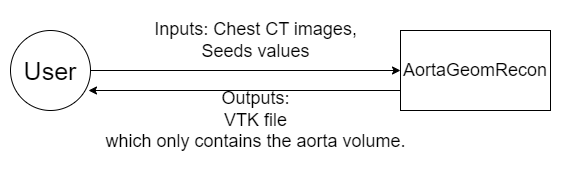
\includegraphics[width=1\textwidth]{AortaSystemContext.png}
\caption{System Context}
\label{Fig_SystemContext} 
\end{center}
\end{figure}


\begin{itemize}
\item User Responsibilities:
\begin{itemize}
\item Provide the input data to the system
\item Ensure the input meets the necessary assumptions
\item Verify the result meets their requirements, otherwise repeat the process with a different seed values.
\end{itemize}
\item \progname{} Responsibilities:
\begin{itemize}
\item Provide DICOM data reader which can take a path to a folder containing DICOM files.
\item Provide crop functionality to easily select a region of interest. 
\item Provide simple interactions to obtain and store the users' inputs. This includes a data probe to read voxel location which stored as a coordinate, and text inputs for real numbers.
\item Provide visualization on the result data.
\end{itemize}
\end{itemize}

\subsection{User Characteristics} \label{SecUserCharacteristics}
The end user of \progname{} should have taken the university level anatomy introduction course, and be capable of finding the center of the descending aorta and the ascending aorta.

\subsection{System Constraints} \label{SecSysConstraints}


\section{Specific System Description}

This section first presents the problem description, which gives a high-level
view of the problem to be solved.  This is followed by the solution characteristics
specification, which presents the assumptions, theories, definitions and finally
the instance models.  

\subsection{Problem Description} \label{Sec_pd}

The main purpose of \progname{} is to semi-automatically segment a 3D aorta geometry from a chest CT scan.

\subsubsection{Organ Segmentation}

Organs are the body's recognizable structures (for example, the heart, lungs, liver, eyes, and stomach) that perform specific functions. Figure \ref{FigHO} below shows all the organs within a human body. The organ segmentation or the organ boundary segmentation is useful for orientation and identification of the regions of interests inside the organ during the diagnostic or treatment procedure. The aorta segmentation is important for aortic calcification quantification and to guide the segmentation of other central vessels. \cite{TissuesAndOrgans}

\begin{figure}[H]
\centering
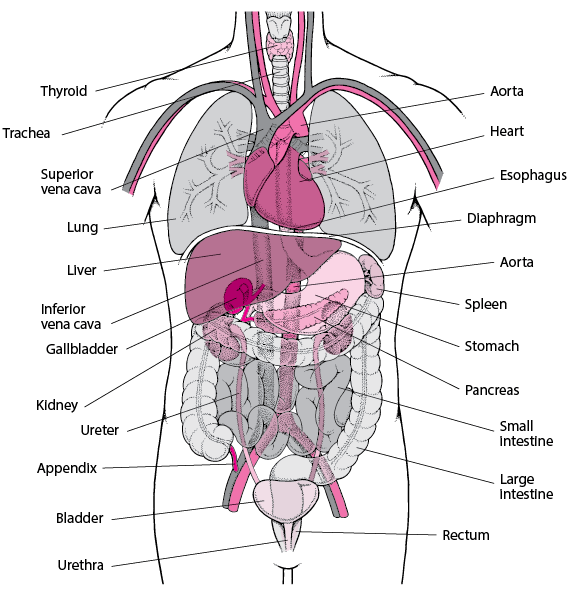
\includegraphics[width=95mm]{humanOrgans}
\caption{Human organs ~\cite{TissuesAndOrgans}}
\label{FigHO}
\end{figure}

\subsubsection{Coordinate Systems}
This subsection provides a list of terms that are used in the subsequent
sections and their meaning, with the purpose of reducing ambiguity and making it
easier to correctly understand the requirements. \cite{Nejad2017} \\

\noindent While working with medical images, it is necessary to be familiar with the different coordinate systems of the medical literarure and how data (voxels' orientation) is interpreted in different medical and non-medical software. Each coordinate system uses one or more numbers (coordinates) to uniquely determine the position of a point (in the medical context, we refer to each point as a voxel). The purpose of this section is to introduce some of the coordinate systems related to the medical imaging. There are different coordinate systems to represent data. A knowledge of the following coordinate systems is needed to work with the medical images.

\paragraph{Cartesian Coordinate System}
A Cartesian coordinate system is a coordinate system that specifies each point uniquely in a 2D plane by a pair of numerical coordinates or in a 3D space by three numerical coordinates. We assume a right-hand Cartesian coordinate system throughout this document.

\paragraph{World Coordinate System}
World Coordinate System (WCS) is a Cartesian coordinate system that describes the physical coordinates associated with a model such as an MRI scanner or a patient. While each model has its own coordinate system, without a universal coordinate system such as WCS, they cannot interact with each other. For model interaction to be possible, their coordinate systems must be transformed into the WCS. Figure \ref{WCS} shows the WCS corresponding space and axes.
\begin{figure}[hbpt!]
\centering
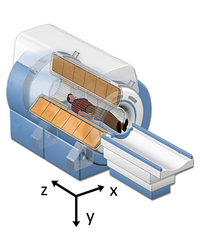
\includegraphics[width=50mm]{worldCoordinateSystem.png}
\caption{World Coordinate System Space and Axes~\cite{slicerWCS}}
\label{WCS}
\end{figure}
\paragraph{Anatomical Coordinate System}
Anatomical coordinate system, also known as patient coordinate system, is a right-handed 3D coordinate system that describes the standard anatomical position of a human using the following 3 orthogonal planes:
\begin{itemize}
\item{Axial / Transverse plane:} is a plane parallel to the ground that separates the body into head (superior) and tail (inferior) positions.
\item{Coronal / Frontal plane:} is a plane perpendicular to the ground that divides the body into front (anterior) and back (posterior) positions.
\item{Sagittal / Median plane:} is a plane that divides the body into right and left positions.
\end{itemize}
Figure \ref{ACS} shows this coordinate system.

\begin{figure}[H] 
\centering
\subfloat[\centering Anatomical Coordinate System]{{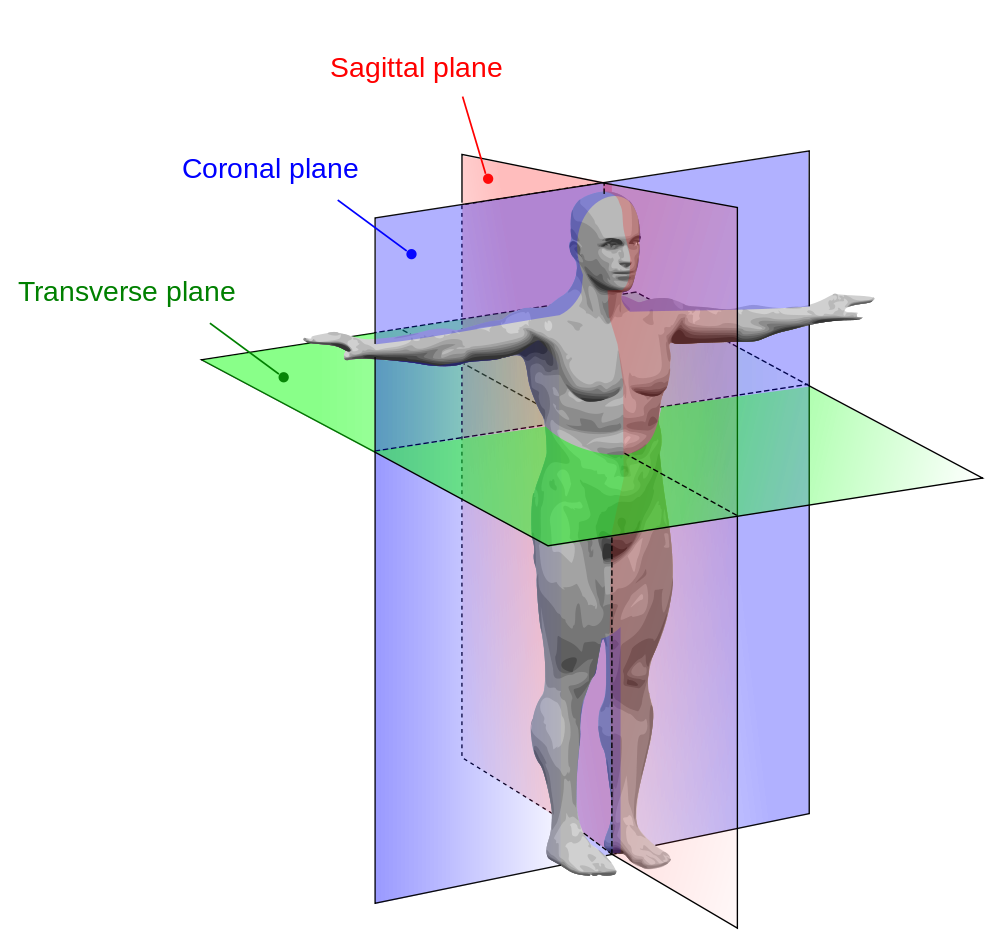
\includegraphics[width=9cm]{anatomicalCoordinateSystem1.png} }}%
\subfloat[\centering Space and Axes]{{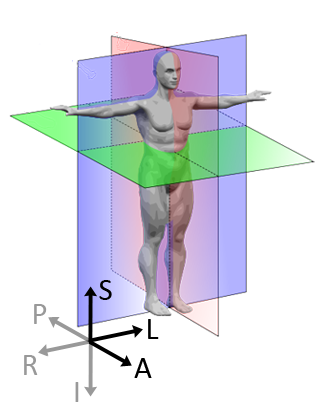
\includegraphics[width=6cm]{anatomicalCoordinateSystem2.png} }}%
\caption{Anatomical Coordinate System Space and Axes~\cite{slicerWCS}} %without this we cannot have label
\label{ACS}
\end{figure}

\noindent Medical applications follow an anatomical coordinate system to store voxels in sequences. Depending on how the data is stored, this coordinate system can be divided into different bases. The most common ones are:
\begin{itemize}
\item{LPS Coordinate System:}

The LPS coordinate system is used in DICOM images. In this system, voxels are ordered from left to right in a row, rows are ordered from posterior to anterior, and slices are stored from inferior to superior.
\indent
LPS stands for Left-Posterior-Superior which indicates the directions that spatial axes are increasing.
% RAI Radiological preferred axes.
\item{RAS Coordinate System:}

The RAS coordinate system is the preferred basis for Neurological applications such as 3dfim+, and 3D Slicer. RAS stands for Right-Anterior-Superior is similar to LPS with the first two axes flipped.
\end{itemize}

\paragraph{Image Coordinate System}
 
To specify locations in an image we need to know to which coordinate system it is referenced. Different software may use different orders as their index convention.

\noindent Each of the coordinate systems mentioned above are used by different systems.

\subsubsection{Physical System Description} \label{sec_phySystDescrip}
We do not study the physical system for the images or how the data is actually generated.

\subsubsection{Goal Statements}

\noindent Given the DICOM image that includes patient's chest,
the descending aorta center voxel coordinate,
and the ascending aorta center voxel coordinate, the goal statements is:

\begin{itemize}

\item[GS\refstepcounter{goalnum}\thegoalnum \label{Gsegment}:] 
Extract the three dimensional segmentation of the aorta.

\end{itemize}

\subsection{Solution Characteristics Specification}

\subsubsection{Assumptions} \label{sec_assumpt}

This section simplifies the original problem and helps in developing the
theoretical model by filling in the missing information for the physical
system. The numbers given in the square brackets refer to the theoretical model
[T], general definition [GD], data definition [DD], instance model [IM], or
likely change [LC], in which the respective assumption is used.

\begin{itemize}
\item[A\refstepcounter{assumpnum}\theassumpnum \label{A_aorta_volume}:]
The 3D image provided by the user must contains a visually distingushable aorta volume [\iref{roi}].

\item[A\refstepcounter{assumpnum}\theassumpnum \label{A_roi}:]
User should select a valid region of interest [\iref{segmentation}].

\end{itemize}

\subsubsection{Theoretical Models}\label{sec_theoretical}
There are no theoretical models used in this document.

\subsubsection{General Definitions}\label{sec_gendef}
There are no general definition used in this document.

\subsubsection{Data Definitions}\label{sec_datadef}
This section collects and defines all the data needed to build the instance
models.

\noindent
\begin{minipage}{\textwidth}
\renewcommand*{\arraystretch}{1.5}
\begin{tabular}{| p{\colAwidth} | p{\colBwidth}|}
\hline
\rowcolor[gray]{0.9}
Number& DD\refstepcounter{datadefnum}\thedatadefnum \label{v}\\
\hline
Label& \bf Voxel \\
\hline
Symbol & $ \textit{v} : \mathbb{R}$\\
\hline
% Units& $Mt^{-3}$\\
% \hline
  SI Units & - \\
  \hline
  Equation& - \\
  \hline
  Description & 
                A slice (\ddref{slice}) consists of $ n \times n$ voxels. A real number is assigned to each voxel to reports the intensity on a grey-scale image.
  \\
  \hline
  Sources & \cite{Nejad2017} \\
  \hline
  Ref.\ By & \ddref{slice}\\
  \hline
\end{tabular}
\end{minipage}\\

% -----------------------------------------------------------------------------------------------------------------------------------------------------------------------------------------------------------------

\noindent
\begin{minipage}{\textwidth}
\renewcommand*{\arraystretch}{1.5}
\begin{tabular}{| p{\colAwidth} | p{\colBwidth}|}
\hline
\rowcolor[gray]{0.9}
Number& DD\refstepcounter{datadefnum}\thedatadefnum \label{slice}\\
\hline
Label& \bf Image/Slice \\
\hline
Symbol & $ \textit{slice} : \mathbb{R}^{m \times n}$\\
\hline
% Units& $Mt^{-3}$\\
% \hline
  SI Units & - \\
  \hline
  Equation& - \\
  \hline
  Description & 
                A visual representation that is using only two spatial dimensions with a sequence of arrays where a voxel (\ddref{v}) represents the color or intensity. Each move in the transverse plane (Figure \ref{ACS}) is considered as one slice
  \\
  \hline
  Sources & \cite{Nejad2017} \\
  \hline
  Ref.\ By & \ddref{volume}\\
  \hline
\end{tabular}
\end{minipage}\\

% -----------------------------------------------------------------------------------------------------------------------------------------------------------------------------------------------------------------

\noindent
\begin{minipage}{\textwidth}
\renewcommand*{\arraystretch}{1.5}
\begin{tabular}{| p{\colAwidth} | p{\colBwidth}|}
\hline
\rowcolor[gray]{0.9}
Number& DD\refstepcounter{datadefnum}\thedatadefnum \label{volume}\\
\hline
Label& \bf Volume\\
\hline
Symbol & $ \textit{V} : \mathbb{R}^{m \times n \times p}$\\
\hline
% Units& $Mt^{-3}$\\
% \hline
  SI Units & - \\
  \hline
  Equation& - \\
  \hline
  Description & A three dimensional image is a sequence of some images/slices (\ddref{slice}).
  \\
  \hline
  Sources & - \\
  \hline
  Ref.\ By & \iref{roi}\\
  \hline
\end{tabular}
\end{minipage}\\

\subsubsection{Data Types}\label{sec_datatypes}
There are no additional data types used in this document.

\subsubsection{Instance Models} \label{sec_instance}    

This section transforms the problem defined in Section~\ref{Sec_pd} into 
one which is expressed in mathematical terms. It uses concrete symbols defined 
in Section~\ref{sec_datadef} to replace the abstract symbols in the models. There are no theoretical models or general definitions used in this document.\\

\noindent 
The goals \gsref{Gsegment} are solved by finding \iref{roi} and perform \iref{segmentation} on the aorta.

~\newline

%Instance Model 1

\noindent
\begin{minipage}{\textwidth}
\renewcommand*{\arraystretch}{1.5}
\begin{tabular}{| p{\colAwidth} | p{\colBwidth}|}
  \hline
  \rowcolor[gray]{0.9}
  Number& IM\refstepcounter{instnum}\theinstnum \label{roi}\\
  \hline
  Label& \bf Region of interest \\
  \hline
  Inputs & $ \textit{V}_\text{in}:\mathbb{R}^{m_i \times n_i \times p_i}$ , $\textit{Start} : \mathbb{N}^3 $, $m_o, n_o, p_o : \mathbb{N}$,  with the following constraints:
\begin{center}
$ 0 \leq Start[0] < (m_i-1) $ \\
$ 0 \leq Start[1] < (n_i-1) $ \\
$ 0 \leq Start[2] < (p_i-1) $ \\
$ 0 < m_o \leq (m_i-Start[0]) $ \\
$ 0 < n_o \leq (n_i-Start[1]) $ \\
$ 0 < p_o \leq (p_i-Start[2]) $ \\
\end{center}\\
  \hline
  Output& $ \textit{V}_\text{out} : \mathbb{R}^{m_o \times n_o \times p_o}$ such that
\begin{center}
$ \forall (i,j,k : \mathbb{N}\text{ } | \text{ }$ \\
$ i \in [Start[0]..Start[0]+m_o] \wedge $ \\
$ j \in [Start[1]..Start[1]+n_o] \wedge $ \\
$ k \in [Start[2]..Start[2]+p_o] :$\\
$ V_\text{out}[i][j][k]=V_\text{in}[i][j][k])$
\end{center}\\
  \hline
  Description & The regions of interest is a subset (shaped like a box) of the 3D $V_{\text{out}}$. This subset contains the anatomical structure that the users wants to read, process or extract. 
  \\
  \hline
  Sources&  \\
  \hline
  Ref.\ By & \iref{segmentation} \\
  \hline
\end{tabular}
\end{minipage}\\

~\newline

%Instance Model 1

\noindent
\begin{minipage}{\textwidth}
\renewcommand*{\arraystretch}{1.5}
\begin{tabular}{| p{\colAwidth} | p{\colBwidth}|}
  \hline
  \rowcolor[gray]{0.9}
  Number& IM\refstepcounter{instnum}\theinstnum \label{segmentation}\\
  \hline
  Label& \bf Segmentation \\
  \hline
  Input & $ V_\text{in} : \mathbb{R}^{m \times n \times p}$, $Seed\_a: \mathbb{N}^{3}$, $Seed\_d: \mathbb{N}^3$ \\
  \hline
  Output& $ V_\text{out} : \mathbb{R}^{m \times n \times p}$ such that
\begin{center}
$ \forall (i,j,k : \mathbb{N} $         $|$ \\
$ i \in [0..m-1] \wedge $ 
$ j \in [0..n-1] \wedge $
$ k \in[0..p-1] :$\\
$ (V_\text{in}[i,j,k] \in \text{structure} \implies V_\text{out}[i,j,k]=HIGH\text{ }|$\\
$ V_\text{in}[i,j,k] \notin \text{structure} \implies V_\text{out}[i,j,k]=LOW)) $ \\
\end{center}
The inputs Seed\_a and Seed\_d are used to determine whether a given element of $V_\text{in}$ is in structure or not.
\\
  \hline
  Description & The process of extract an anotomical structure from the original 3D volume. The extracted anotomical structure is represented with high intensity pixel value. The rest of the image should have a lower intensity pixel value. The segmentation needs the region of interset from \iref{roi} to process less noise data. A seed is what the algorithm needed as the inputs to perform segmentation, the type of a seed is different among different algorithm. The seeds in this section are the centre coordinate of the descending aorta and the ascending aorta. The yellow dots shown in Figure \ref{AortaSeeds} are the example of the seed.\\
  \hline
  Sources& \\
  \hline
  Ref.\ By & \rref{R_output}, \lcref{LC_seg_algorithm}\\
  \hline
\end{tabular}
\end{minipage}

\begin{figure}[H]
\centering
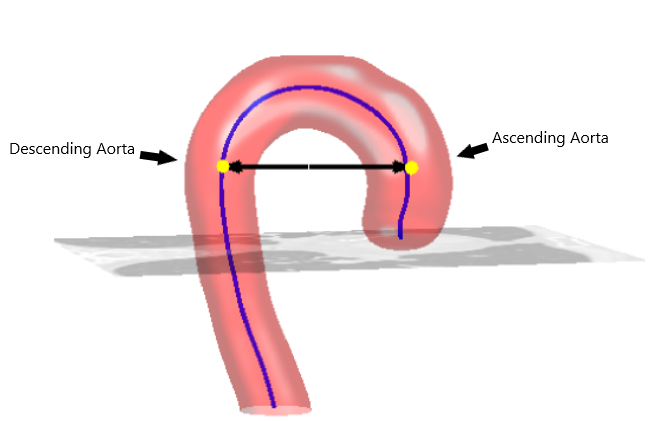
\includegraphics[width=120mm]{Aorta_seeds}
\caption{Aorta Seeds} \label{AortaSeeds} 
\end{figure} 

\subsubsection{Input Data Constraints} \label{sec_DataConstraints}    
The only software constraint is the input volume data. It must be an acceptable file type to the system processing the data. For example, using ITK-Snap software to perform organ segmentation, the input data must be of VTK file.

\subsubsection{Properties of a Correct Solution} \label{sec_CorrectSolution}

\noindent
A correct solution cannot be measured, but it can be confirmed by visually comparing the intersection of the extracted anotomical structure and the original volume.

\section{Requirements}

This section provides the functional requirements, the business tasks that the
software is expected to complete, and the nonfunctional requirements, the
qualities that the software is expected to exhibit.

\subsection{Functional Requirements}

\noindent \begin{itemize}
\item[R\refstepcounter{reqnum}\thereqnum \label{R_Inputs}:] Input the following
  functions, data and parameters:
  \renewcommand{\arraystretch}{1.2}
%\noindent \begin{tabularx}{1.0\textwidth}{l l X}
  \noindent \begin{longtable*}{l l p{12cm}} \toprule
         \textbf{symbol}  & \textbf{description}\\
         \midrule 
$V$ & CT Scans volume
(\ddref{volume})\\ %comparing value used for excluding correlation coefficients
$Seed\_a$ & The seed of ascending aorta centre coordinate (\iref{segmentation})\\
$Seed\_d$ & The seed of descending aorta centre coordinate (\iref{segmentation})\\
         \bottomrule
\end{longtable*}

\item[R\refstepcounter{reqnum}\thereqnum \label{R_roi}:] Use the volume in \rref{R_Inputs} to create a second volume, the region of interest (\iref{roi}) that contains all of the aorta.

\item[R\refstepcounter{reqnum}\thereqnum \label{R_output}:] Perform segmentation (\iref{segmentation}) on the volume created in \rref{R_roi}.

\item[R\refstepcounter{reqnum}\thereqnum \label{R_visualize}:] Visualize a volume (\ddref{volume}).

\end{itemize}

\subsection{Nonfunctional Requirements}

\noindent \begin{itemize}

\item[NFR\refstepcounter{nfrnum}\thenfrnum \label{NFR_GUI}:] \textbf{Usability}
\progname{} provides a user-friendly interface to import any DICOM files, and input the required parameters.

\item[NFR\refstepcounter{nfrnum}\thenfrnum \label{NFR_Safety}:] \textbf{Safety}
For a valid image, the \progname{} provides a correct solution, or no answer.

\item[NFR\refstepcounter{nfrnum}\thenfrnum \label{NFR_Learnability}:] \textbf{Learnability}
The user interface and documentation should allow a user that meets the user characteristics (Section \ref{SecUserCharacteristics}) to learn how to do an aorta segmentation in at least 30\% of the time it takes to learn and use ITK-Snap (bubble method mentioned in Section \ref{intro}).

\item[NFR\refstepcounter{nfrnum}\thenfrnum \label{NFR_Accuracy}:] \textbf{Accuracy}
For a given image the segmentation found by \progname{} should match that found by an expert using ITK-Snap. Whether to two segmentations match is something that would be judged by a medical imaging expert.

\item[NFR\refstepcounter{nfrnum}\thenfrnum \label{NFR_Consistency}:] \textbf{Consistency}
The coordinate system may be modified through the calculations, but any transformations will not alter the meaning of the data.

%\item[NFR\refstepcounter{nfrnum}\thenfrnum \label{NFR_visualize}:] \textbf{Usability}
%\progname{} can visualize the volume with 3D rendering.


\item Other NFRs that might be discussed include verifiability, and reusability.

\end{itemize}

\section{Likely Changes}    

\noindent \begin{itemize}

\item[LC\refstepcounter{lcnum}\thelcnum\label{LC_seg_algorithm}:] \iref{segmentation} There are various segmentation algorithms, each has a different procedure and inputs.
	
\end{itemize}

\section{Unlikely Changes}    

\noindent \begin{itemize}

\item[UC\refstepcounter{ucnum}\theucnum\label{UC_roi}:] \iref{roi} The method to retrieve a region of interest from a volume is fixed.
	
\end{itemize}


\section{Traceability Matrices and Graphs}

The purpose of the traceability matrices is to provide easy references on what
has to be additionally modified if a certain component is changed.  Every time a
component is changed, the items in the column of that component that are marked
with an ``X'' may have to be modified as well.  Table~\ref{Table:trace} shows the
dependencies of theoretical models, general definitions, data definitions, and
instance models with each other. Table~\ref{Table:R_trace} shows the
dependencies of instance models, requirements, and data constraints on each
other. Table~\ref{Table:A_trace} shows the dependencies of theoretical models,
general definitions, data definitions, instance models, and likely changes on
the assumptions.\\

\noindent The purpose of the traceability graphs is also to provide easy references on
what has to be additionally modified if a certain component is changed.  The
arrows in the graphs represent dependencies. The component at the tail of an
arrow is depended on by the component at the head of that arrow. Therefore, if a
component is changed, the components that it points to should also be
changed.

\begin{table}[H]
\centering
\begin{tabular}{|c|c|c|c|c|c|}
\hline        
	& \ddref{v} & \ddref{slice} & \ddref{volume} & \iref{roi} &  \iref{segmentation} \\
\hline
\ddref{v}     & &  & & & \\ \hline
\ddref{slice}    & X & & & &\\ \hline
\ddref{volume}    & & X & & & \\ \hline
\iref{roi}        & & & X & & \\ \hline
\iref{segmentation}      &  & & & X & \\
\hline
\end{tabular}
\caption{Traceability Matrix Showing the Connections Between Items of Different Sections}
\label{Table:trace}
\end{table}

\begin{table}[H]
\centering
\begin{tabular}{|c|c|c|c|c|c|c|c|c|c|c|c|}
\hline
	& \iref{roi}& \iref{segmentation}& \rref{R_Inputs}& \rref{R_roi}& \rref{R_output} & \rref{R_visualize} & \nfrref{NFR_GUI} & \nfrref{NFR_Safety} & \nfrref{NFR_Learnability} & \nfrref{NFR_Accuracy} & \nfrref{NFR_Consistency} \\
\hline
\iref{roi}            & & & & X & & &  & & & &\\ \hline
\iref{segmentation}  & & & & & X & &  & & & &\\ \hline
\rref{R_Inputs}       & & X & & & & & & & & &\\ \hline
\rref{R_roi}   & X & & & & & & & & & &\\ \hline
\rref{R_output}  & & X & & & & & & & & &\\ \hline
\rref{R_visualize}  & & & & & & & X & & & &\\ \hline
\nfrref{NFR_GUI} & & & X & X & X & X & & & X & &\\ \hline
\nfrref{NFR_Safety}   & & X &  &  &  &  & & & & &\\ \hline
\nfrref{NFR_Learnability} & & & & X & X & X & X & & & & \\ \hline
\nfrref{NFR_Accuracy} & & X & & & & & & & & &\\ \hline
\nfrref{NFR_Consistency} & & X & & & & & & & & &\\ \hline
\end{tabular}
\caption{Traceability Matrix Showing the Connections Between Requirements and Instance Models}
\label{Table:R_trace}
\end{table}

\begin{table}[H]
\centering
\begin{tabular}{|c|c|c|}
\hline
	& \aref{A_aorta_volume}& \aref{A_roi} \\
\hline
\ddref{v}                     & & \\ \hline
\ddref{slice}                 & & \\ \hline
\ddref{volume}             & & \\ \hline
\iref{roi}                       &X & \\ \hline
\iref{segmentation}        & &X \\ \hline
\lcref{LC_seg_algorithm} &X &X\\ \hline
\ucref{UC_roi}               & & \\ \hline
\end{tabular}
\caption{Traceability Matrix Showing the Connections Between Assumptions and Other Items}
\label{Table:A_trace}
\end{table}

\newpage

\section{Referance}
\bibliographystyle {plainnat}
\bibliography {../../refs/References}

\end{document}